
\chapter{付録}

%\section{deconvolutionの計算}
%\section{駆動系の電気信号}
%\section{GaAsの発振}
%線形離島の領域なの?
\section{リッジ導波路型レーザーにおいて観測されたドループに関する追加実験}

本節ではリッジ導波路型レーザーのILカーブ測定で観測されたドループを軽減する方法を模索するために行った実験について述べる。ドループは試料の温度上昇によるものだと考え、活性層部分の熱が逃げやすいよう上下をひっくり返してサブマントにダイボンディングを行った。このマウント方法をエピダウンと呼ぶ。その写真を図\ref{fig:fig_5_1_epidown_mount}に示す。写真は3周期歪量子井戸レーザー$L=300\ \si{\micro\metre}$である。裏向きの試料がALNサブマウントに大ボンディングされている。図では試料のn側コンタクトが見えており、そこから出たワイヤーがプローバーでさわるためのパターンに配線されている。このマウント方法は活性層がサブマウント、サブマウントが乗っている銅板に近いため熱が逃げやすい。
\begin{figure}[h]
	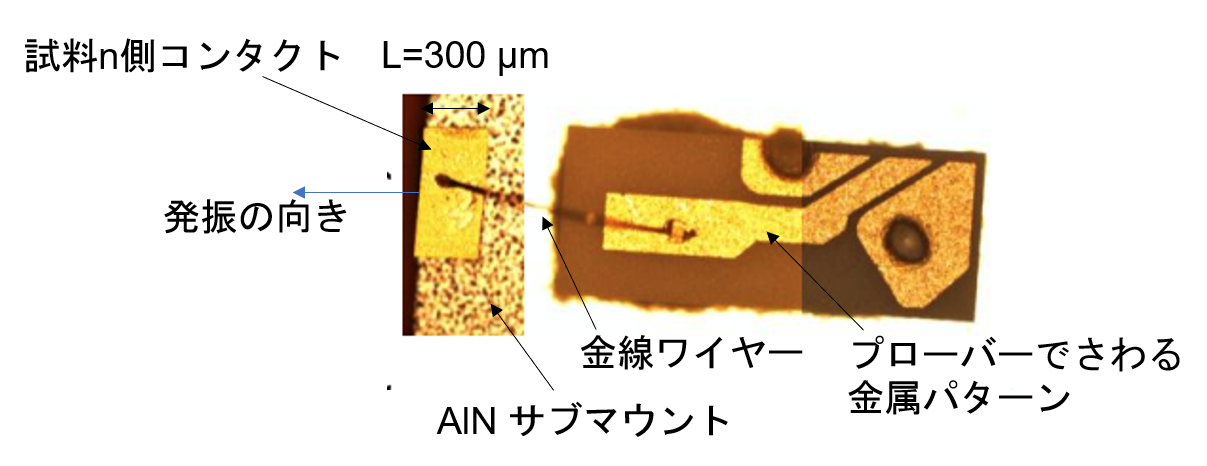
\includegraphics[width=15cm]{figure/fig_5_1_epidown_mount.png}
	\caption{エピダウン試料マウントの様子}
	\label{fig:fig_5_1_epidown_mount}
\end{figure}


図\ref{fig:fig_5_1_epidown_IL}にエピダウン試料の定常電流注入実験結果のILカーブを示す。測定は全て2\ $\si{\micro s}$パルスを2\ $\si{m s}$周期で印加しており(デュティー比1:1000)、プロットは片側端面からの発光強度を1000倍した値である。試料は全て3周期歪量子井戸リッジ導波路型レーザーの結果である。

まず、破線はエピダウンを行っていない3周期試料($L=500\ \si{\micro\metre}$)のILカーブであり、色分けは同じ試料に対する測定回数を表す。1回目の測定では200\ \si{mA}程度まで電流を流した結果、ドループは見られなかった。2回目の測定では300\ \si{mA}まで電流を流すとドループが観測された。さらに測定を重ねて行うと発光量はさらに少なくなっていく様子が見られた。

次に実線及び点線のプロットはエピダウンを行った試料のILカーブを示す。色分けはそれぞれ共振器長を表している。これらの試料では$L=300, 400 \ \si{\micro\metre}$では電流400\ mAで発光強度が60\ mWとエピダウンしていない試料よりも高い値を持っている。また、$L=1000\ \si{\micro\metre}$においては電流1000\ mAまで流してもドループは見られず80\ mW程度までの発光が確認された。

この実験からエピダウンにより活性層の温度上昇が抑制されまたドループも抑制されることがわかった。
\begin{figure}[h]
	\centering
	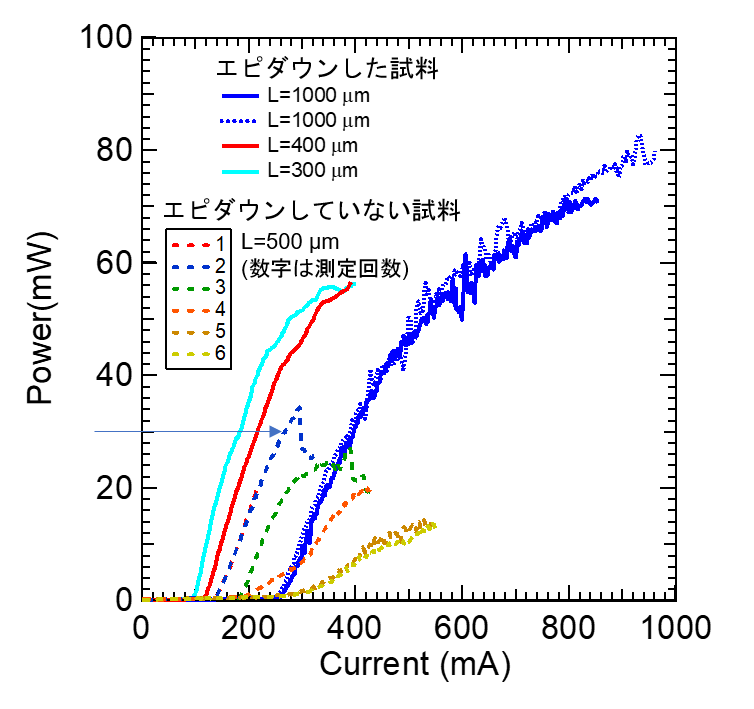
\includegraphics[width=10cm]{figure/fig_5_1_epidown_IL.png}
	\caption{エピダウン試料のILカーブ}
	\label{fig:fig_5_1_epidown_IL}
\end{figure}

%\clearpage
\section{リッジ導波路型レーザーにおけるFIB加工レーザー試料の測定}
本節ではFIB加工(集束イオンビーム、Focused Ion Beam)を用いた試料作製とその結果について示す。
ブロードコンタクトレーザー試料の測定結果からキャリアがパッド幅方向(リッジ導波路型レーザーにおいてはリッジ幅方向)にキャリアが広がっている可能性が示唆されていた。そこでFIB加工によりリッジの両脇に活性層よりも十分深い溝を形成しキャリアの拡散が起こらないような試料を作製し、定常電流注入実験を行った。実験には3周期歪量子井戸リッジ導波路型レーザー($L=300\ \si{\micro\metre}$)を用いた。またFIB加工はNTT-AT社に外注した。

図\ref{fig:fig_5_2_FIB_facet}にFIB加工を行った試料の端面方向の写真を示す。リッジの両側に深い溝が形成されていることがわかる。
溝の幅は$6\sim17\ \si{\micro\metre}$の試料を作製した。
\begin{figure}[h]
	\centering
	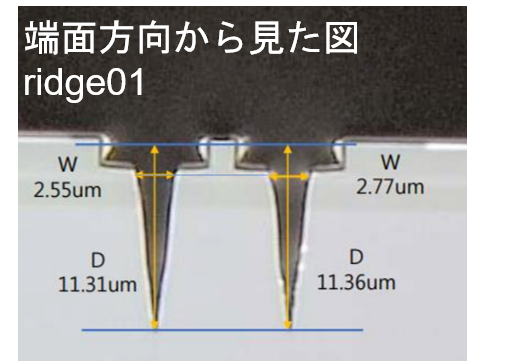
\includegraphics[width=8cm]{figure/fig_5_2_FIB_facet.png}
	\caption{FIB試料の端面写真}
	\label{fig:fig_5_2_FIB_facet}
\end{figure}


図\ref{fig:fig_5_2_FIB_IL}にFIB加工試料の定常電流注入測定結果のILカーブを示す。これを見ると閾値電流は最小で60 mA程度とFIB加工を行っていない試料の結果(図\ref{fig:fig_3_2_3QW_ridge_IL}及び図\ref{fig:fig_3_2_3QW_ridge_Ith}では最小80 mA)と比較すると小さくなっている。FIB加工による電流の流れる幅を制限したことにより閾値低減が行われたことがわかる。このことから電流が広がって流れているのではないかと考察される。
\begin{figure}[h]
	\centering
	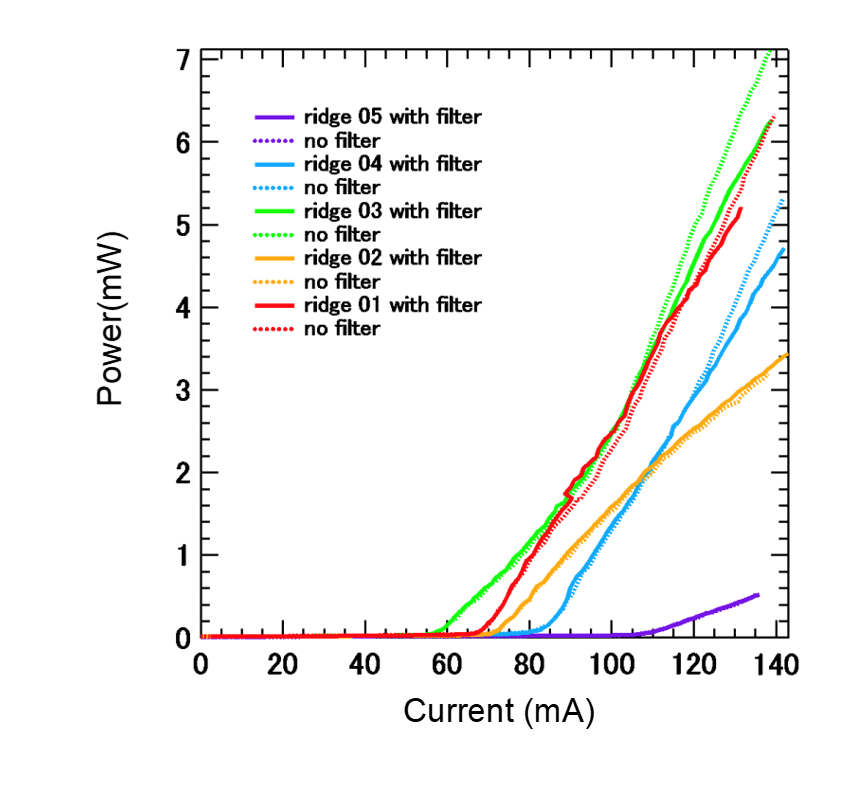
\includegraphics[width=10cm]{figure/fig_5_2_FIB_IL.png}
	\caption{FIB試料のILカーブ}
	\label{fig:fig_5_2_FIB_IL}
\end{figure}



\clearpage
\section{格子定数、$E_{g}$の計算}
$\rm{In_{1-x}Ga_{x}As_{y}P_{1-x}}$の格子状数は\cite{ref_iga}より
\begin{eqnarray}
a=5.8687-0.4176x+0.1896y+0.0125xy\\
\end{eqnarray}
と計算した。$\rm{Al_{1-x}Ga{x}As}$の格子定数は
\begin{eqnarray}
a=5.65325x+5.6605(1-x)
\end{eqnarray}
として計算した。
$E_{g}$は下の表の式を用いて計算を行った。
\begin{table}[h]
  \caption{3周期歪量子井戸ブロードコンタクトレーザーの電流広がり}
  \label{table:table_Eg}
  \centering
  \begin{tabular}{cc}
    \hline
    材料& $E_{g}$の式   \\
    \hline \hline
     $\rm{Ga_{x}In_{1-x}As}$ &$0.324+0.7x+0.4x^2$   \\
    $\rm{Al_{x}Ga_{1-x}As}$& $1.420+1.087x+0.438x^2$ \\
    $\rm{Ga_{x}In_{1-x}P}$& $1.351+0.643x+0.786x^2$ \\ 
    $\rm{GaAs_{x}P_{1-x}}$&$2.750-1.502x+0.176x^2$\\
    \hline
  \end{tabular}
\end{table}
%\subsection{InGaPのトンネル}

